\documentclass[conference,10pt]{IEEEtran}
\IEEEoverridecommandlockouts
\usepackage[T1]{fontenc}
\usepackage{amsmath,amssymb}
\usepackage{booktabs}
\usepackage{multirow}
\usepackage{graphicx}
\usepackage{algorithm}
\usepackage[noend]{algpseudocode}
\usepackage{tikz}
\usetikzlibrary{positioning,arrows.meta,calc}
\usepackage{pgfplots}
\pgfplotsset{compat=1.18}
\usepackage[hidelinks]{hyperref}
\usepackage{xspace}

% Every evaluation number below is a macro generated by paper/eval_ci.py from
% backend/mayajaal/mirage/eval_results.json (committed run) and a 2,000-seed rerun.
% generated by paper/eval_ci.py -- do not edit by hand
\newcommand{\NSeedsCI}{2{,}000}
\newcommand{\NSeedsCommitted}{500}
\newcommand{\MaxSteps}{30}
\newcommand{\CMMirageSteps}{17.50}
\newcommand{\CMMirageReach}{71.9}
\newcommand{\CMMirageAcc}{57.8}
\newcommand{\EMMirageSteps}{17.35\,$\pm$\,0.18}
\newcommand{\EMMirageReach}{73.1\,$\pm$\,0.9}
\newcommand{\EMMirageAcc}{58.2\,$\pm$\,0.9}
\newcommand{\CMRandomSteps}{18.75}
\newcommand{\CMRandomReach}{69.7}
\newcommand{\CMRandomAcc}{54.4}
\newcommand{\EMRandomSteps}{18.72\,$\pm$\,0.18}
\newcommand{\EMRandomReach}{70.1\,$\pm$\,0.9}
\newcommand{\EMRandomAcc}{54.5\,$\pm$\,0.9}
\newcommand{\CMNoneSteps}{21.46}
\newcommand{\CMNoneReach}{61.9}
\newcommand{\CMNoneAcc}{46.2}
\newcommand{\EMNoneSteps}{21.31\,$\pm$\,0.16}
\newcommand{\EMNoneReach}{62.5\,$\pm$\,0.9}
\newcommand{\EMNoneAcc}{46.9\,$\pm$\,0.9}
\newcommand{\DMMvNSteps}{\ensuremath{-}3.95\,$\pm$\,0.16}
\newcommand{\DMMvNReach}{10.6\,$\pm$\,0.7}
\newcommand{\DMMvNAcc}{11.3\,$\pm$\,0.9}
\newcommand{\DMMvRSteps}{\ensuremath{-}1.36\,$\pm$\,0.16}
\newcommand{\DMMvRReach}{3.0\,$\pm$\,0.7}
\newcommand{\DMMvRAcc}{3.7\,$\pm$\,0.9}
\newcommand{\DMRvNSteps}{\ensuremath{-}2.59\,$\pm$\,0.14}
\newcommand{\DMRvNReach}{7.6\,$\pm$\,0.7}
\newcommand{\DMRvNAcc}{7.6\,$\pm$\,0.8}
\newcommand{\EMBenignDiv}{1.7\,$\pm$\,0.6}
\newcommand{\EMBenignCrumbs}{0.044}
\newcommand{\CXMirageSteps}{19.20}
\newcommand{\CXMirageReach}{65.9}
\newcommand{\CXMirageAcc}{49.5}
\newcommand{\EXMirageSteps}{19.22\,$\pm$\,0.19}
\newcommand{\EXMirageReach}{66.9\,$\pm$\,0.9}
\newcommand{\EXMirageAcc}{50.0\,$\pm$\,0.9}
\newcommand{\CXRandomSteps}{19.96}
\newcommand{\CXRandomReach}{65.0}
\newcommand{\CXRandomAcc}{48.7}
\newcommand{\EXRandomSteps}{19.98\,$\pm$\,0.18}
\newcommand{\EXRandomReach}{65.5\,$\pm$\,0.9}
\newcommand{\EXRandomAcc}{49.0\,$\pm$\,0.9}
\newcommand{\CXNoneSteps}{21.46}
\newcommand{\CXNoneReach}{61.9}
\newcommand{\CXNoneAcc}{46.2}
\newcommand{\EXNoneSteps}{21.31\,$\pm$\,0.16}
\newcommand{\EXNoneReach}{62.5\,$\pm$\,0.9}
\newcommand{\EXNoneAcc}{46.9\,$\pm$\,0.9}
\newcommand{\DXMvNSteps}{\ensuremath{-}2.08\,$\pm$\,0.16}
\newcommand{\DXMvNReach}{4.4\,$\pm$\,0.7}
\newcommand{\DXMvNAcc}{3.1\,$\pm$\,0.9}
\newcommand{\DXMvRSteps}{\ensuremath{-}0.76\,$\pm$\,0.18}
\newcommand{\DXMvRReach}{1.4\,$\pm$\,0.8}
\newcommand{\DXMvRAcc}{1.0\,$\pm$\,1.0}
\newcommand{\DXRvNSteps}{\ensuremath{-}1.32\,$\pm$\,0.14}
\newcommand{\DXRvNReach}{3.0\,$\pm$\,0.7}
\newcommand{\DXRvNAcc}{2.2\,$\pm$\,0.8}
\newcommand{\EXBenignDiv}{1.7\,$\pm$\,0.6}
\newcommand{\EXBenignCrumbs}{0.044}
\newcommand{\CMBenignDiv}{1.6}
\newcommand{\CMBenignCrumbs}{0.04}
\newcommand{\CMIGRecon}{0.171}
\newcommand{\CRIGRecon}{0.137}
\newcommand{\CMStepsRecon}{10.34}
\newcommand{\CNStepsRecon}{14.70}
\newcommand{\CMReachRecon}{96.0}
\newcommand{\CNReachRecon}{94.2}
\newcommand{\CMIGExfil}{0.218}
\newcommand{\CRIGExfil}{0.169}
\newcommand{\CMStepsExfil}{21.15}
\newcommand{\CNStepsExfil}{27.05}
\newcommand{\CMReachExfil}{49.6}
\newcommand{\CNReachExfil}{24.0}
\newcommand{\CMIGTamper}{0.215}
\newcommand{\CRIGTamper}{0.155}
\newcommand{\CMStepsTamper}{14.56}
\newcommand{\CNStepsTamper}{19.04}
\newcommand{\CMReachTamper}{91.8}
\newcommand{\CNReachTamper}{83.8}
\newcommand{\CMIGDisrupt}{0.184}
\newcommand{\CRIGDisrupt}{0.145}
\newcommand{\CMStepsDisrupt}{23.97}
\newcommand{\CNStepsDisrupt}{25.06}
\newcommand{\CMReachDisrupt}{50.0}
\newcommand{\CNReachDisrupt}{45.6}


\newcommand{\Mirage}{\textsc{Mirage}\xspace}
\newcommand{\code}[1]{\texttt{\small #1}}
\newcommand{\pb}{p_{\mathrm{b}}}
\DeclareMathOperator*{\argmax}{arg\,max}
\algrenewcommand\algorithmicrequire{\textbf{Input:}}
\algrenewcommand\algorithmiccomment[1]{\hfill$\triangleright$ #1}

\begin{document}

\title{\Mirage: Adaptive Session-Seeded Deception\\for Hospital APIs}
\author{\IEEEauthorblockN{MayaJaal --- HackPrinceton Fall 2026}}
\maketitle

\begin{abstract}
MayaJaal puts a gateway in front of a hospital's FHIR API and IT portal. When a signed-in session
starts to act like an intruder, its non-clinical traffic is silently moved into a synthetic
``shadow'' hospital generated from a per-session HMAC seed, while real records stay behind the
policy. \Mirage is the adaptive layer of this system. It has three parts: a Bayesian filter over
the session's goal and kill-chain stage; a lane adjuster that can only make treatment stricter; and
a breadcrumb planner that plants the lure whose take/ignore outcome has the highest expected
information gain about the goal. In an in-model simulation against a simulated attacker policy,
averaged over four attack goals, max-gain lures cut the mean number of requests needed to put
$>0.8$ posterior on the true goal from \CMNoneSteps{} (no lures) to \CMMirageSteps{}, compared
with \CMRandomSteps{} for random lures. The advantage shrinks when engagement is misspecified. We
report no human red-team data.
\end{abstract}

\section{Introduction}
In June 2024 a ransomware attack on Synnovis, the pathology provider for several south-east London
NHS trusts, disrupted blood testing and forced the postponement of planned
care~\cite{nhs2024synnovis}. An intruder holding one valid login can do real harm, but a hospital
cannot simply cut access when it is unsure, because clinicians need records to treat patients.

Deception suits this setting. A decoy wastes the intruder's time, reveals intent and raises a
high-signal alarm~\cite{cohen1998deception,spitzner2002honeypots}. Static honeypots, however, look
the same to every visitor, so their artefacts can be fingerprinted and the fingerprints
shared~\cite{holz2005detecting,vetterl2018bitter}. Work on decoy documents and honeywords shows
that per-user, plausible bait is much harder to tell from the real
thing~\cite{bowen2009baiting,juels2013honeywords}. MayaJaal gives each diverted session its own
deterministic shadow hospital. \Mirage then decides, from what the session appears to want, which
lures to add to that hospital. Our contributions: (i)~a lane policy with sticky diversion in which
clinical reads are stepped up or denied but never faked; (ii)~a tempered (goal$\times$stage)
filter that reaches the policy only through a monotone lane raise; (iii)~a max-information-gain
lure planner that sees only the goal posterior; (iv)~a reproducible simulation with confidence
intervals.

\section{Threat Model}
The adversary holds valid credentials for a clinical account (in our scenario, a phished nurse) and
reaches the hospital over HTTP through the FHIR API and the IT portal. It may be an autonomous
agent. Its goal is \emph{recon}, \emph{exfil} (bulk records or backups), \emph{tamper} (lab
results) or \emph{disrupt}. The defender wins if none of the 12 protected canary secrets seeded into
the real tier leaves through the gateway. Ten of them sit in restricted notes at hospitals other
than the phished user's own; the other two are an SSN and a service API secret. We assume the
gateway, the policy engine and the shadow key are not compromised. Timing side channels,
comparison across several accounts and attacks on the host are out of scope (\S\ref{sec:limits}).

\section{Method}

\begin{figure}[t]
\centering
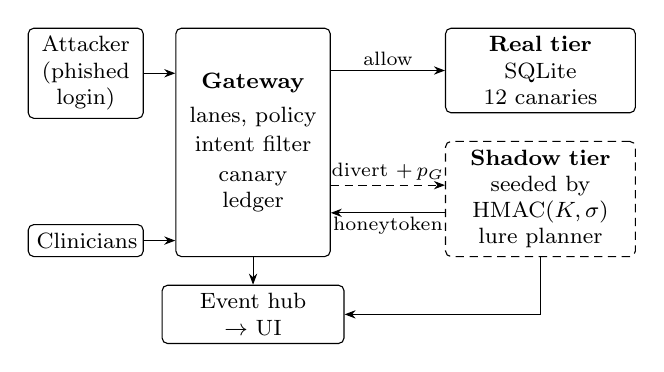
\begin{tikzpicture}[font=\footnotesize, >={Stealth[length=4pt]},
  box/.style={draw, rounded corners=2pt, align=center, inner sep=3pt},
  lab/.style={font=\scriptsize, align=center, inner sep=1.5pt}]
\node[box, text width=1.75cm, minimum height=2.9cm] (gw) {\textbf{Gateway}\\[3pt]lanes, policy\\[1pt]intent filter\\[1pt]canary ledger};
\node[box, text width=1.25cm, left=0.4cm of gw.north west, anchor=north east] (att) {Attacker\\(phished login)};
\node[box, text width=1.25cm, left=0.4cm of gw.south west, anchor=south east] (cli) {Clinicians};
\node[box, text width=2.2cm, right=1.45cm of gw.north east, anchor=north west] (real) {\textbf{Real tier}\\SQLite\\12 canaries};
\node[box, text width=2.2cm, right=1.45cm of gw.south east, anchor=south west, densely dashed] (sh)
     {\textbf{Shadow tier}\\seeded by HMAC$(K,\sigma)$\\lure planner};
\node[box, text width=2.1cm, below=0.35cm of gw] (hub) {Event hub $\to$ UI};
\draw[->] (att.east) -- (att.east -| gw.west);
\draw[->] (cli.east) -- (cli.east -| gw.west);
\draw[->] (gw.east |- real.west) -- node[lab, above]{allow} (real.west);
\draw[->, densely dashed] ([yshift=5pt]gw.east |- sh.west) -- node[lab, above]{divert $+\,p_G$} ([yshift=5pt]sh.west);
\draw[<-] ([yshift=-5pt]gw.east |- sh.west) -- node[lab, below]{honeytoken} ([yshift=-5pt]sh.west);
\draw[->] (gw) -- (hub);
\draw[->] (sh.south) |- (hub.east);
\end{tikzpicture}
\caption{Architecture. The gateway is the only public port. Clinical reads from a suspect session
are refused (401 step-up or 403) and never served from the shadow. The shadow process has no code
path or file path to the real tier and receives only the goal posterior $p_G$ in a header.
Responses to non-clinician callers are scanned for canaries.}
\label{fig:arch}
\end{figure}

\subsection{Gateway lanes and sticky diversion}
Each session has a lane $\ell\in\{\textit{normal}<\textit{suspicious}<\textit{attacker}\}$ (or
\textit{unauth} with no token) and a \emph{diverted} bit. Requests are classified as clinical
read, list or write, bulk export, admin, backup or other. Fixed signals raise the lane: admin or
backup access by a non-admin, a bulk export ($\code{\_count}>100$ or \code{\$export}) from an
interactive role, cross-hospital enumeration or reads, and lab writes by roles that do not write
labs. A honeytoken touch sets \textit{attacker}. The gateway stores the decided lane, so an
authenticated session's lane never decreases. The action is a lookup
$a=\textsc{Act}[\text{bucket}][\ell]$. Sensitive buckets (backup, admin, export, clinical write,
cross-hospital list) are diverted from \textit{suspicious} upward. Clinical reads get
\code{step\_up} (401) when \textit{suspicious} and \code{deny} (403) when \textit{attacker}, so a
misclassified clinician never acts on a fake chart. The one exception is an identifier that does
not exist in the real tier, such as a shadow honeytoken MRN, which may be diverted. Diversion is
\emph{sticky}: once a session is diverted, every non-clinical request that would have been allowed
is diverted too, so the session sees one consistent world. The static-honeypot baseline seeds the
shadow with a fixed string, so every visitor sees the same decoy.

\subsection{Intent filter}
The hidden state is $(g,s)$, with goal $g\in\{\text{b(enign)},\text{recon},\text{exfil},\text{tamper},
\text{disrupt}\}$ and stage $s\in(\text{recon},\text{access},\text{collect},\text{act})$. The prior
is $b_0(g,s)=\pi(g)\rho(s)$, with $\pi=(.80,.08,.05,.04,.03)$ and $\rho=(.70,.20,.08,.02)$.

\emph{Predict.} Let $m_g=\sum_s b(g,s)$ and $q_g=b(g,\cdot)/m_g$. Stages only move forward:
$q'_g=q_gA$, where $A$ advances a stage with probability $\alpha=0.15$ and \emph{act} is absorbing.
Goals are sticky. An attack goal keeps a fraction $1-\delta$ of its mass ($\delta=0.04$), and a
benign session turns hostile with probability $\tau=0.005$. The mass that switches is spread over
attack goals in proportion to $\pi_A(g)\propto\pi(g)$ and enters at the stage prior:
\begin{align}
\bar b(g,s)&=m_g(1-\delta_g)\,q'_g(s)+\iota_g\,\rho(s),\label{eq:pred}\\
\iota_g&=\big(\delta(1-m_\text{b})+\tau m_\text{b}\big)\pi_A(g),\nonumber
\end{align}
where $\delta_\text{b}=\tau$ and $\iota_\text{b}=0$. No mass ever flows back to benign, so only
evidence can clear a session.

\emph{Likelihood.} Each request maps to one of 22 categories $c$ (ward list, cross-hospital list,
record read, note read, bulk export, lab write, backup, admin page, \dots) and two flags $f$:
\emph{denied} (401/403) and \emph{honeytoken}. A hand-written table gives goal weights $W_{c,g}$
and stage multipliers $M_{c,s}$; benign sessions have no stage:
\begin{equation}
P(c\mid g,s)\propto W_{c,g}\,M_{c,s}^{[g\neq\text{b}]}\quad\text{(normalised over $c$).}\label{eq:lik}
\end{equation}
Flags have tables $P(f\mid g)$. Only a flag that is present counts as evidence.

\emph{Update.} Requests are correlated, so evidence is tempered by $\gamma=0.7$ and the $k$-th
consecutive repeat of a category is further scaled by $1/\sqrt{k}$:
\begin{multline}
b_t(g,s)\propto\bar b(g,s)\,P(c_t\mid g,s)^{\gamma/\sqrt{k_t}}\prod_{f\in F_t}P(f\mid g)^{\gamma}\\
\cdot\big[E_{\kappa g}^{\,o}(1-E_{\kappa g})^{1-o}\big].\label{eq:upd}
\end{multline}
The bracketed term applies only when a lure $\kappa$ was planted and its outcome $o\in\{0,1\}$ is
seen, with $E_{\kappa g}=P(\text{engage}\mid g,\kappa)$. The live gateway sees an engagement only
as a honeytoken flag; the explicit form is used offline. The goal posterior is
$p_G(g)=\sum_s b_t(g,s)$. Unit tests check that a simulated 150-request nurse stays above $0.9$
benign throughout, and that a scripted exfiltration run ends with exfil between $0.78$ and $0.95$
rather than near $1$.

\subsection{Monotone lane adjustment}
The filter affects routing only through $\ell\leftarrow\max(\ell,\lambda(\pb))$. Here
$\pb=p_G(\text{b})$ is taken after the \emph{previous} request, and $\lambda$ returns
\textit{attacker} if $\pb<0.10$, \textit{suspicious} if $\pb<0.35$, and no change otherwise.
\textit{Unauth} is left alone. For every bucket, access to the real tier does not increase as
$\ell$ rises. A wrong or manipulated posterior can therefore make the gateway stricter, but it can
never grant access that the rules refuse.

\subsection{Information-gain breadcrumb planning}
The planner runs in the shadow process. Its only input from the gateway is $p_G$, rounded to three
decimals and sent in the \code{X-MJ-Posterior} header on diverted requests. There are five lure
kinds: a backup share, an admin credential, a research dataset, a lab service account and a VPN
config. Each has hand-set rates $E_{\kappa g}$; for example, exfil takes a backup dump with
probability 0.85 and tamper with 0.15. The planner chooses
\begin{equation}
\kappa^\star=\argmax_{\kappa\in\mathcal K\setminus\mathcal P}\;
H(G)-\sum_{o\in\{0,1\}}P(o\mid\kappa)\,H(G\mid o,\kappa),\label{eq:ig}
\end{equation}
where $P(o{=}1\mid\kappa)=\sum_g E_{\kappa g}p_G(g)$ and
$P(g\mid o,\kappa)\propto P(o\mid g,\kappa)\,p_G(g)$. This is the exact expected entropy
reduction, i.e.\ the mutual information between goal and
outcome~\cite{lindley1956measure,cover2006elements}. $\mathcal P$ is the set of lures already
planted. A lure is planted only in a non-static world, at most once every 4 requests, at most 3
times per session, and only when the gain is at least $0.03$ bits. Each lure carries freshly minted
honeytokens. The choice is greedy and looks one step ahead; it is not a full sequential design.

\subsection{Session-seeded shadow generation}
Every shadow entity $e$ (a patient, lab panel, dump, file, honeytoken or lure) draws from a PRNG
seeded with $\mathrm{HMAC\text{-}SHA256}(K,\sigma\|\text{``}|\text{''}\|e)$~\cite{rfc2104}, where
$\sigma$ is the session id and $K$ is a 32-byte process key. The world is generated lazily and has
no fixed size, but it is deterministic: an id always returns the same patient, a dump's rows match
\code{GET /Patient}, and different sessions get different hospitals. A per-session overlay records
the attacker's writes. Honeytoken ids are derived the same way, so a token seen anywhere points to
the session that read it. Only public templates (name lists, code tables) are used. Tests scan the
source and inspect \code{sys.modules} at runtime to confirm that the shadow tier never imports
\code{mayajaal.real} and never reads its data.
\emph{Canary ledger.} Each response body sent to a non-clinician caller is gunzipped if needed and
searched for every canary in case-folded form, as hex, and as base64 at all three byte alignments.
Leak counts are kept per run and only increase.

\begin{algorithm}[t]
\caption{Per-request handling for session $\sigma$}\label{alg:req}
\begin{algorithmic}[1]
\footnotesize
\Require lane $\ell$, diverted bit $d$, belief $b$, shadow world $W_\sigma$
\State $c\gets\textsc{Classify}(\text{req})$; $\ell\gets\max(\ell,\textsc{Signal}(c,\text{role}))$
\State $\ell\gets\max(\ell,\lambda(p_G(\text{b})))$ \Comment{monotone; $b$ from step $t{-}1$}
\State $a\gets\textsc{Act}[\textsc{Bucket}(c)][\ell]$
\State \textbf{if} $d\wedge a{=}\text{allow}\wedge c$ non-clinical \textbf{then} $a\gets\text{divert}$
\If{$a=\text{allow}$} serve from the real tier
\ElsIf{$a=\text{divert}$}
  \State $d\gets$ true; forward to $W_\sigma$ with header $p_G$
  \State \textbf{if} gates pass \textbf{then} plant $\kappa^\star$ of \eqref{eq:ig} in $W_\sigma$
  \State \textbf{if} honeytoken touched \textbf{then} $\ell\gets\textit{attacker}$
\Else{} 401 step-up or 403 \Comment{clinical data never faked}
\EndIf
\State \textsc{Ledger.Scan}(response)
\State $b\gets\textsc{Update}(\textsc{Predict}(b),\textsc{Features}(\text{req}))$ \Comment{\eqref{eq:pred}--\eqref{eq:upd}}
\end{algorithmic}
\end{algorithm}

\section{Evaluation}
\textbf{Setup.} \code{mayajaal.mirage.evaluate} is an \emph{in-model simulation against a simulated
attacker policy}. It uses no human red-team data and does not measure real agents. For each true
goal and seed, the stage starts at recon and advances with probability 0.2 per request. Each
request category is drawn from $0.5\,P(c\mid g,s)+0.5\,P_{\text{gen}}(c)$, where $P_\text{gen}$ is a
goal-agnostic mix of portal pages, lists, record reads and discovery. Routine traffic is
therefore weaker evidence than the filter assumes. Benign sessions draw from
$P(c\mid\text{b})$. A session counts as diverted once $\pb<0.35$, and lures are planted only after
that. A lure is taken on the next request with probability $E_{\kappa g}$ (\emph{matched}) or
$0.5E_{\kappa g}+0.2$ (\emph{misspecified}). Three strategies are compared: max-IG, a uniformly
random unplanted kind under the same gates, and no lures. All three see the same request stream for
a given seed. The metrics are the number of requests until $p_G(g^\star)>0.8$ (censored at
\MaxSteps, so a restricted mean), the share of sessions that reach $0.8$, and top-goal accuracy at
request 10. The committed \code{eval\_results.json} (\NSeedsCommitted{} seeds per cell) is
reproduced exactly by rerunning the module. For intervals, \code{paper/eval\_ci.py} calls the
unchanged \code{run\_session} with \NSeedsCI{} seeds per cell. It reports 95\% normal intervals,
stratified across the four attack goals, with differences paired by seed.

\begin{table}[t]
\centering
\caption{Attack-goal averages. ``500'': committed run. Other columns: \NSeedsCI{} seeds, 95\% CI.
Simulation of our own model.}
\label{tab:res}
\footnotesize
\setlength{\tabcolsep}{3.2pt}
\begin{tabular}{@{}l@{\hspace{6pt}}lcccc@{}}
\toprule
 \multicolumn{2}{@{}l}{Lures} & \multicolumn{2}{c}{Steps to 0.8 $\downarrow$} & Reached (\%) & Acc@10 (\%)\\
\cmidrule(lr){3-4}
 & & 500 & 95\% CI & 95\% CI & 95\% CI\\
\midrule
\multicolumn{6}{@{}l}{\emph{matched engagement}}\\
 & max-IG & \CMMirageSteps & \EMMirageSteps & \EMMirageReach & \EMMirageAcc\\
 & random & \CMRandomSteps & \EMRandomSteps & \EMRandomReach & \EMRandomAcc\\
 & none   & \CMNoneSteps   & \EMNoneSteps   & \EMNoneReach   & \EMNoneAcc\\
\multicolumn{6}{@{}l}{\emph{misspecified engagement}}\\
 & max-IG & \CXMirageSteps & \EXMirageSteps & \EXMirageReach & \EXMirageAcc\\
 & random & \CXRandomSteps & \EXRandomSteps & \EXRandomReach & \EXRandomAcc\\
\bottomrule
\end{tabular}
\end{table}

\begin{figure}[t]
\centering
\begin{tikzpicture}
\begin{axis}[
  width=\columnwidth, height=3.8cm,
  ybar, bar width=7pt, ymin=0, ymax=34, enlarge x limits=0.15,
  xtick=data, xticklabels={recon,exfil,tamper,disrupt},
  ylabel={requests}, ylabel style={font=\footnotesize},
  tick label style={font=\footnotesize}, ytick={0,10,20,30},
  legend style={font=\footnotesize, draw=none, fill=none, at={(0.5,1.02)}, anchor=south,
                legend columns=3, /tikz/every even column/.append style={column sep=6pt}},
  legend image code/.code={\draw[#1] (0cm,-0.08cm) rectangle (0.22cm,0.12cm);},
  error bars/y dir=both, error bars/y explicit,
  axis x line*=bottom, axis y line*=left]
\addplot[fill=black, draw=black] table[x=idx, y=mirage, y error=mirageci] {data/steps_by_goal.dat};
\addplot[fill=gray!50, draw=black] table[x=idx, y=random, y error=randomci] {data/steps_by_goal.dat};
\addplot[fill=white, draw=black] table[x=idx, y=none, y error=noneci] {data/steps_by_goal.dat};
\legend{max-IG, random, none}
\end{axis}
\end{tikzpicture}
\caption{Mean requests until the true goal's posterior exceeds 0.8 (censored at \MaxSteps; lower is
better). Matched engagement, \NSeedsCI{} seeds, 95\% CI. Simulation of our own model.}
\label{fig:goals}
\end{figure}

\textbf{Results.} See Table~\ref{tab:res} and Fig.~\ref{fig:goals}. With matched engagement and
paired by seed, max-IG lures change the step count by \DMMvNSteps{} relative to no lures, and
random lures by \DMRvNSteps. Compared directly with random lures, max-IG changes steps by
\DMMvRSteps{} and accuracy at request 10 by \DMMvRAcc{} points. Lures chosen by max-IG also carry
more expected information than random ones: in the committed run they average \CMIGExfil{} vs.\
\CRIGExfil{} bits in exfil sessions and \CMIGTamper{} vs.\ \CRIGTamper{} in tamper sessions.
Exfil benefits most: the share of sessions that reach 0.8 rises from \CNReachExfil\% with no lures
to \CMReachExfil\% with max-IG. When engagement is misspecified, max-IG still beats no lures
(\DXMvNSteps{} steps). Its lead over random falls to \DXMvRSteps{} steps, and the accuracy
difference (\DXMvRAcc{} points) is barely significant. Disrupt remains hard under every strategy
(\CMReachDisrupt\% reach 0.8 with max-IG) because its request profile overlaps with recon.
Of the simulated benign sessions, \EMBenignDiv\% are diverted (\CMBenignDiv\% in the committed run).
Under the rule table, those sessions lose non-clinical surfaces, but their clinical reads are
still never faked.

\section{Limitations and Ethics}\label{sec:limits}
\textbf{The evaluation is circular by design.} Requests are drawn, with added noise, from the same
tables the filter uses. The simulation checks the planner's logic. It does not show that the
tables describe real intruders or LLM agents. Every value in $W$, $M$, $E$ and the thresholds is a
judgement call, and none was fitted to data. The planner is greedy, ignores stage, and gains only
about 0.2 bits per lure. \textbf{Detectability.} Two accounts used side by side see two different
hospitals. The step-up on clinical reads is an observable change, and proxying to a second process
may add latency. \textbf{Ledger.} The ledger catches verbatim, case-changed, hex and base64 copies.
It does not catch a canary that is split across responses, encrypted or paraphrased.
\textbf{False positives.} A clinician wrongly flagged is stepped up or denied but is never shown
false clinical data. Legitimate non-clinical work, such as an export, can still be silently
diverted, so every diversion needs human review. \textbf{Ethics.} By construction the shadow holds
no real patient data, and each honeytoken is scoped to one session. The system defends a
hospital's own perimeter. It does not identify the attacker, and nothing here shows that it would
have stopped a real incident.

\section{Conclusion}
\Mirage pairs a small, inspectable Bayesian intent model with a gateway in which that model can
only tighten treatment. It spends a small lure budget where the expected information about the
attacker's goal is largest. When we simulate its own model, it identifies attack goals faster than
random lures or none, and the margin narrows under misspecified engagement. The next steps are to
fit the tables to logged red-team and agent runs and to measure detectability directly.

\begin{thebibliography}{10}
\footnotesize
\setlength{\itemsep}{0pt}
\bibitem{nhs2024synnovis} NHS England, statements on the Synnovis cyber incident affecting
south-east London NHS trusts, Jun.\ 2024.
\bibitem{cohen1998deception} F.~Cohen, ``A note on the role of deception in information
protection,'' \emph{Computers \& Security}, vol.~17, no.~6, pp.~483--506, 1998.
\bibitem{spitzner2002honeypots} L.~Spitzner, \emph{Honeypots: Tracking Hackers}. Addison-Wesley,
2002.
\bibitem{holz2005detecting} T.~Holz and F.~Raynal, ``Detecting honeypots and other suspicious
environments,'' in \emph{Proc.\ IEEE SMC Information Assurance Workshop}, 2005.
\bibitem{vetterl2018bitter} A.~Vetterl and R.~Clayton, ``Bitter harvest: Systematically
fingerprinting low- and medium-interaction honeypots at Internet scale,'' in \emph{Proc.\ USENIX
WOOT}, 2018.
\bibitem{bowen2009baiting} B.~M. Bowen, S.~Hershkop, A.~D. Keromytis, and S.~J. Stolfo, ``Baiting
inside attackers using decoy documents,'' in \emph{Proc.\ SecureComm}, 2009.
\bibitem{juels2013honeywords} A.~Juels and R.~L. Rivest, ``Honeywords: Making password-cracking
detectable,'' in \emph{Proc.\ ACM CCS}, 2013.
\bibitem{lindley1956measure} D.~V. Lindley, ``On a measure of the information provided by an
experiment,'' \emph{Ann.\ Math.\ Statist.}, vol.~27, no.~4, pp.~986--1005, 1956.
\bibitem{cover2006elements} T.~M. Cover and J.~A. Thomas, \emph{Elements of Information Theory},
2nd~ed. Wiley, 2006.
\bibitem{rfc2104} H.~Krawczyk, M.~Bellare, and R.~Canetti, ``HMAC: Keyed-hashing for message
authentication,'' RFC~2104, 1997.
\end{thebibliography}

\end{document}
